% !TeX root = ./poster.tex
% The MIT License (MIT)
% =====================

% **Copyright (c) 2018 Anish Athalye (me@anishathalye.com)**

% Permission is hereby granted, free of charge, to any person obtaining a copy of
% this software and associated documentation files (the "Software"), to deal in
% the Software without restriction, including without limitation the rights to
% use, copy, modify, merge, publish, distribute, sublicense, and/or sell copies
% of the Software, and to permit persons to whom the Software is furnished to do
% so, subject to the following conditions:

% The above copyright notice and this permission notice shall be included in all
% copies or substantial portions of the Software.

% THE SOFTWARE IS PROVIDED "AS IS", WITHOUT WARRANTY OF ANY KIND, EXPRESS OR
% IMPLIED, INCLUDING BUT NOT LIMITED TO THE WARRANTIES OF MERCHANTABILITY,
% FITNESS FOR A PARTICULAR PURPOSE AND NONINFRINGEMENT. IN NO EVENT SHALL THE
% AUTHORS OR COPYRIGHT HOLDERS BE LIABLE FOR ANY CLAIM, DAMAGES OR OTHER
% LIABILITY, WHETHER IN AN ACTION OF CONTRACT, TORT OR OTHERWISE, ARISING FROM,
% OUT OF OR IN CONNECTION WITH THE SOFTWARE OR THE USE OR OTHER DEALINGS IN THE
% SOFTWARE.


% Gemini theme
% https://github.com/anishathalye/gemini

\documentclass[final]{beamer}

% ====================
% Packages
% ====================

\usepackage[T1]{fontenc}
\usepackage{lmodern}
\usepackage[size=custom,width=130 ,height=100,scale=1.0]{beamerposter}
\usetheme{gemini}
\usecolortheme{gemini}
\usepackage{graphicx}
\usepackage{booktabs}
\usepackage{tikz}
\usepackage{pgfplots}
\usepackage{tcolorbox}
\usepackage{geometry}

% ====================
% Lengths
% ====================

% If you have N columns, choose \sepwidth and \colwidth such that
% (N+1)*\sepwidth + N*\colwidth = \paperwidth
\newlength{\sepwidth}
\newlength{\colwidth}
\setlength{\sepwidth}{0.025\paperwidth}
\setlength{\colwidth}{0.3\paperwidth}

\newcommand{\separatorcolumn}{\begin{column}{\sepwidth}\end{column}}

% ====================
% Title
% ====================

\title{Ileum microbiota composition and inflammatory response\\ in triple transgenic mice modelling Alzheimer's disease}

\author{Kathryn Conn \textsuperscript{*} \and Christopher R. Keefe \textsuperscript{*} \and Emily Borsom \and Allyson Hirsh \and Melanie Palma Avila \and J. Gregory Caporaso \textsuperscript{†} \and Emily K. Cope \textsuperscript{†} }

\institute[shortinst]{The Pathogen and Microbiome Institute at Northern Arizona University \\
{\footnotesize \textsuperscript{*} Equal Contributors \hskip .5cm \textsuperscript{†} Advisors} }

% ====================
% Body
% ====================

\begin{document}

\begin{frame}[t]
\begin{columns}[t]
\separatorcolumn

\begin{column}{\colwidth}

% TODO: remove
% \begin{block}{Abstract}
%   Alzheimer’s disease (AD), a neurodegenerative disease that affects 1 in 10
%   adults over 65 in the United States, is characterized by neuroinflammation,
%   neurofibrillary tangles, and aggregated amyloid-β plaques in the brain.
%   These key pathologies lead to debilitating symptoms including impaired
%   cognitive function and memory loss. Recent studies indicate a correlation
%   between the gut microbiota and AD, which may be due to mechanisms such as
%   increased inflammatory responses that aggravate neuroinflammation. The gut
%   microbiota is the aggregate of all microbial life resident in the
%   gastrointestinal tract. This bidirectional communication between gut
%   microbes and the brain is known as the gut microbiota-brain axis. By
%   identifying the microbial communities resident in the ileum of triple
%   transgenic mice modeling AD pathologies (3xTg-AD), we can understand
%   correlations between key microbial taxa and AD pathogenesis. In this
%   research, we evaluated the ileum microbiota and inflammatory responses of
%   triple transgenic AD mice compared to wild-type control mice. The ileum is
%   the most distal region of the small intestine and a known site for immune
%   modulation due to the presence of lymph nodules known as Peyer’s patches.
%   Analysis of ileum microbiota composition was performed by sequencing the V4
%   region of the 16S rRNA gene. Microbiome bioinformatics was performed using
%   QIIME 2. Inflammatory responses were quantified using reverse transcriptase
%   quantitative polymerase chain reaction (RT-qPCR) with targeted gene primers
%   and statistical analysis was performed using Prism. We expect to see mice
%   genetically predisposed to developing AD pathologies exhibit a decreased
%   species richness and altered composition of the ileum microbiome and
%   upregulation of proinflammatory cytokines. These studies will provide a
%   critical link between the ileum microbiome, inflammation, and AD, and will
%   contribute to development of microbiota-based therapeutics for AD.
% \end{block}

\begin{block}{Objective and Introduction}

    \textbf{Objective:} To correlate features of the microbial communities
    resident in the ileum of triple transgenic mice modeling AD pathologies
    (3xTg-AD) with Alzheimer's Disease (AD) pathogenesis.

    \textbf{Relevant Context:}
    \begin{itemize}
      \item AD is a neurodegenerative disease that affects 1 in 10 adults over 65 in the United States
      \item The gut microbiota is the aggregate of all microbial life resident in the gastrointestinal tract.
      \item The ileum, the most distal region of the small intestine, is a known site for immune modulation
      \item Studies correlate gut microbiome characteristics and AD pathology, possibly facilitated by bidirectional communication between gut microbes and the brain along the 'gut-brain axis'
      \item AD is characterized by neuroinflammation, neurofibrillary tangles, and aggregated amyloid-β plaques in the brain.
      \item These pathologies may be influenced by inflammatory cytokines produced in the gut.
    \end{itemize}

    \textbf{Hypothesis:}
    We expect to see mice genetically predisposed to developing AD
    pathologies exhibit a decreased species richness and altered composition
    of the ileum microbiome and upregulation of proinflammatory cytokines.
      
  \end{block}

  \begin{block}{Laboratory Methods}

    Here's some filler text about RNA, mice, and samples on ice.

   \begin{tcolorbox}
   [width=\textwidth, colframe=blue]
   {Here's some background stuff in a callout box:}
    \begin{itemize}
      \item {followed by}
      \item {some}
      \item {bullet points}
    \end{itemize}
    \end{tcolorbox}
  \end{block}

  \begin{block}{Bioinformatics Methods}

    TODO: Deal with references
    TODO: Unioned prov DAG if we need to fill space

    Analysis of 16s rRNA data was performed with QIIME 2 2020.2
    (Bolyen et al. 2019). Raw sequence data were demultiplexed and quality
    filtered using the \code{q2‐demux} plugin followed by denoising with
    DADA2 (Callahan et al. 2016) (via \code{q2‐dada2}). A phylogeny was built
    by inserting resulting amplicon sequence variants (ASVs) into a reference
    database constructed from greengenes 13\_8 using the SEPP algorithm (via
   \code{q2‐fragment-insertion}). ASVs were assigned taxonomic annotations from
   the Greengenes 13\_8 99\% OTUs reference sequences (McDonald et al. 2012)
   using \code{q2‐feature‐classifier classify-sklearn} (Bokulich et al.
   2018a)

    .... ETC
    
    TODO: diversity details, longitudinal. Rarefaction depth is up to date.
    Alpha‐diversity metrics (TODO: name Figure methods), beta diversity
    metrics (TODO: name Figure methods), and Principle Coordinate Analysis
    (PCoA) were estimated using q2‐diversity after samples were rarefied
    (subsampled without replacement) to 13102 sequences per sample.

  \end{block}

\end{column}

\separatorcolumn

\begin{column}{\colwidth}

  \begin{block}{Visualizations}
    \begin{figure}[tph!]
      {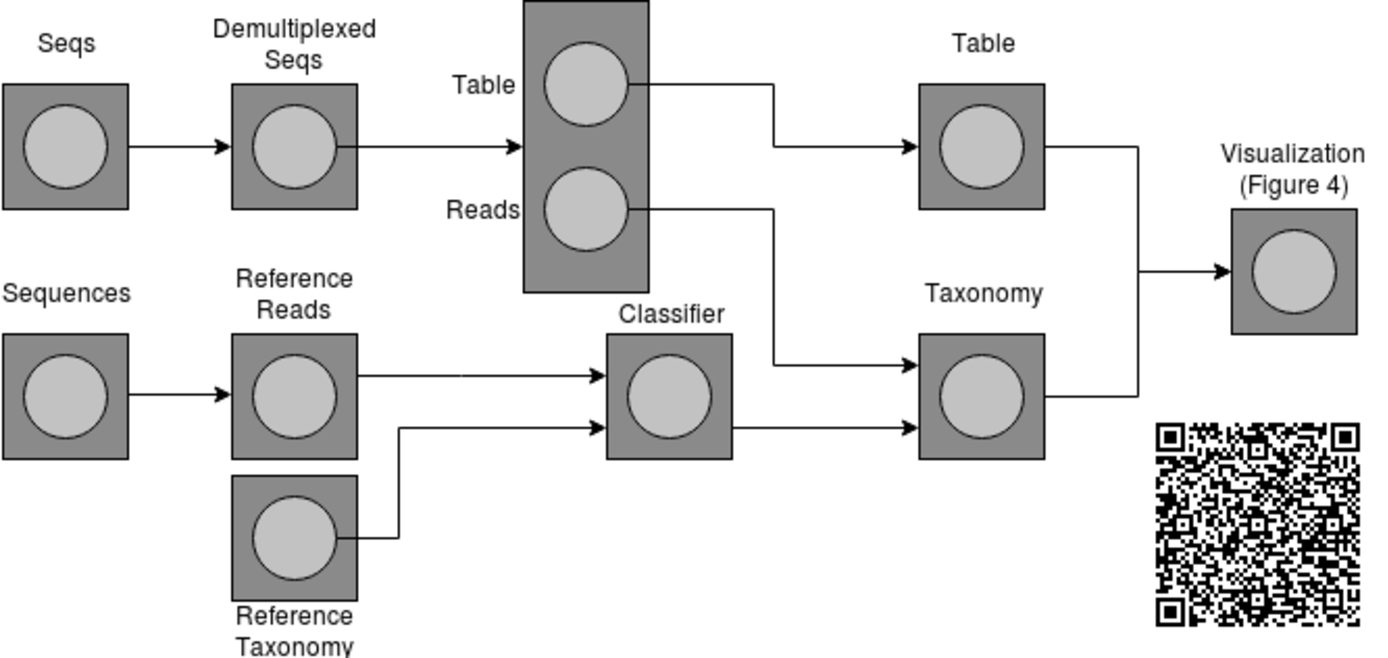
\includegraphics[height=14cm]{assets/provenance}}
      \caption{\,Provenance tree describing the production of our taxonomic bar plot visualization. QR code provides interactive access to both provenance tree and bar plot (Figure 4).}
      \label{fig:provenance}
    \end{figure}

    \begin{figure}[tph!]
      {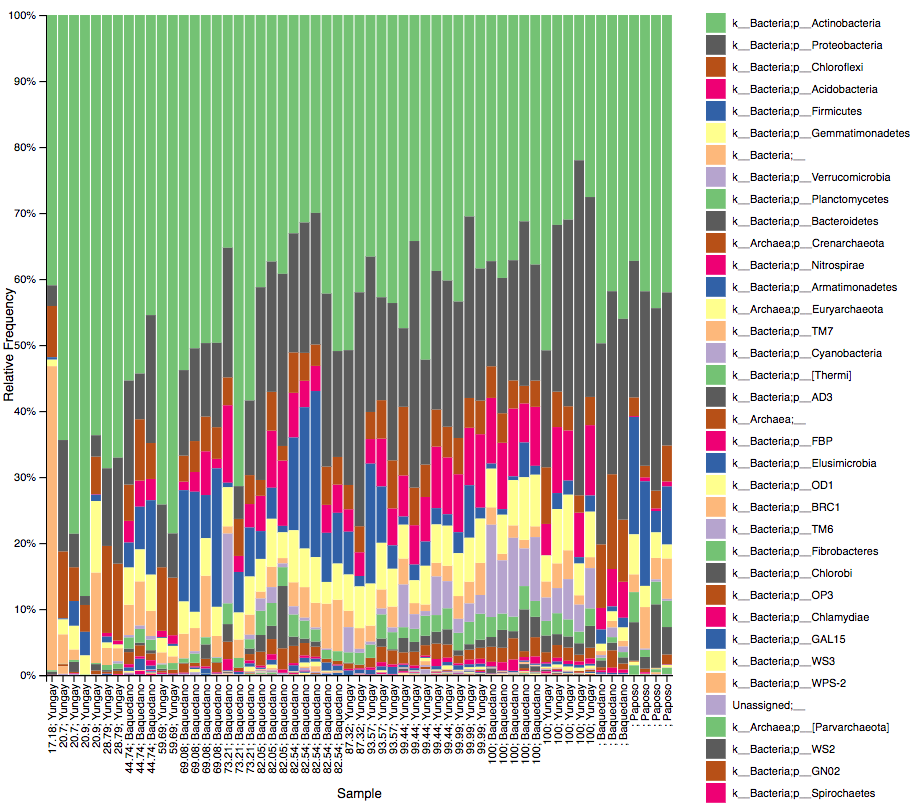
\includegraphics[height=20cm]{assets/taxabar-plot}}
      \caption{\,Taxonomic bar plot sorted by Average Soil Relative Humidity on the x-axis }
      \label{fig:taxabar-plot}
    \end{figure}

    \begin{figure}[tph!]
      {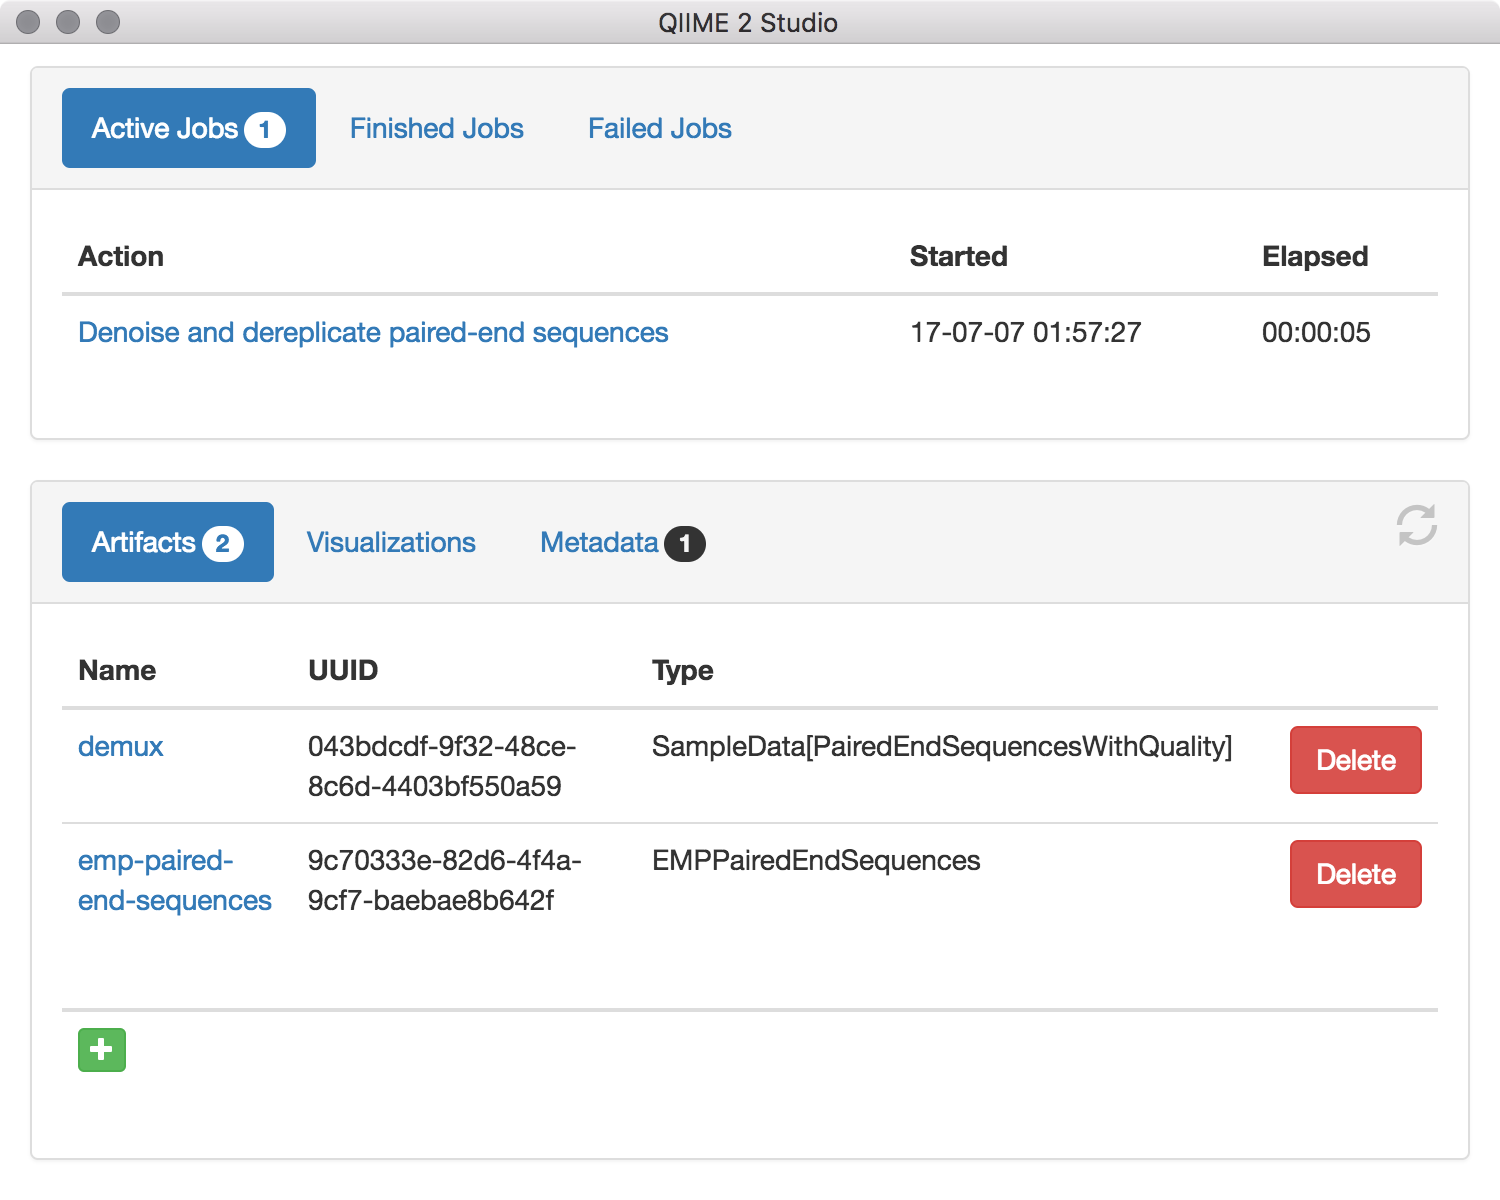
\includegraphics[height=18cm]{assets/q2studio}}
      \caption{\,QIIME 2 Studio provides GUI access to all QIIME 2 plugins installed in the currently active QIIME 2 environment}
      \label{fig:q2studio}
    \end{figure}
  \end{block}

  \begin{block}{Project Funding}
    This work was supported in part by the 2020-21 Urdea Collaborative
    Research Award Program to Kathryn Conn and Chris Keefe, through the
    Northern Arizona University Office of Undergraduate Research \& Creative
    Activity, and by the Arizona Alzheimer’s Consortium (Award number
    CTR040636) to Emily Cope and Greg Caporaso.
  \end{block}
\end{column}

\separatorcolumn

\begin{column}{\colwidth}
    \begin{block}{Results}
      Here are some things we learned from 16s:

      \begin{itemize}
        \item Critters are cool
        \item Mice are nice
        \item Bacteria are bomb
      \end{itemize}

      Here are some things we learned from qPCR:

      \begin{itemize}
        \item Critters are cool
        \item Mice are nice
        \item Bacteria are bomb
      \end{itemize}

    \begin{tcolorbox}
    [width=\textwidth, colframe=blue]
    {A comment on the above results}.
    \end{tcolorbox}

    \begin{figure}[tph!]
      {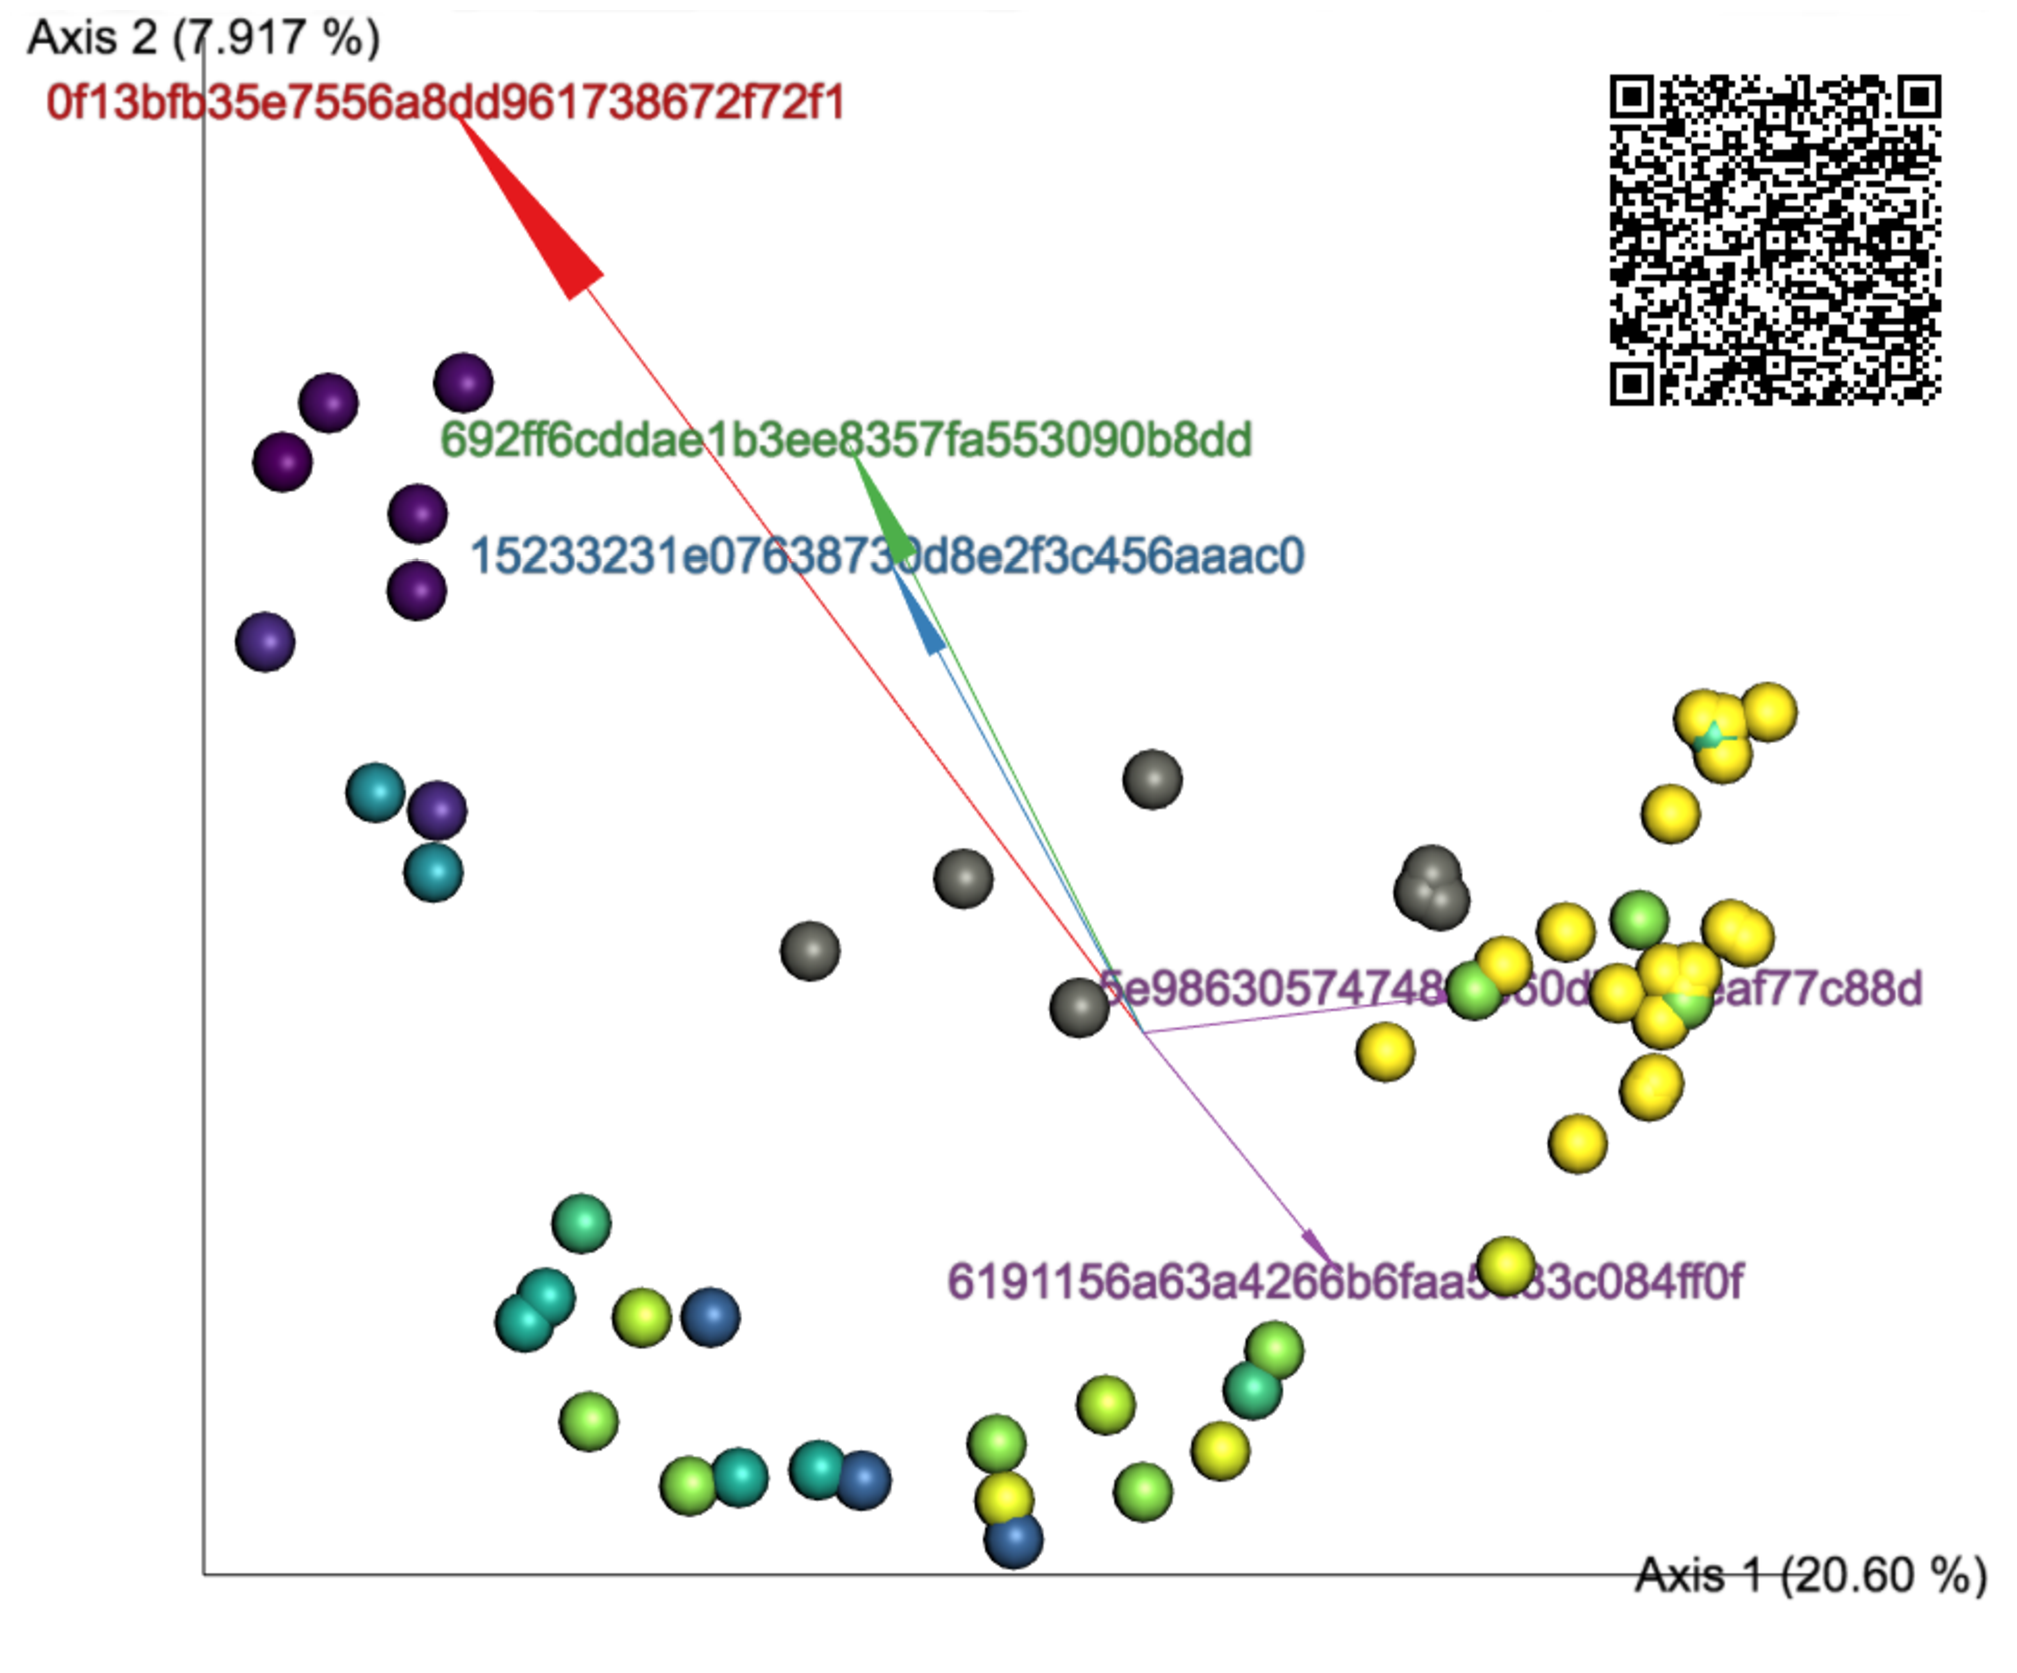
\includegraphics[height=17cm]{assets/emperor}}
      \caption{\,Color gradient represents Average Soil Relative Humidity, with purple ≈ 18 and yellow = 100. Vector colors represent independent clades. \\ \\The magnitude and direction of a vector represents the relative contribution of a given amplicon sequence variant (ASV) to the distance between samples (points). Red: Unknown Bacteria ASV (Kingdom), Green: Bacteria (Kingdom) Actinobacteria (Phylum) Actinobacteria (Class), Blue: Bacteria (Kingdom) Actinobacteria (Phylum) Acidimicrobiia (Class), Purple: Bacteria (Kingdom) Proteobacteria (Phylum) Gammaproteobacteria (Class)}
      \label{fig:emperor}
    \end{figure}

  \end{block}

  \begin{block}{Discussion}

    Though complete longitudinal data are not yet available, the results
    above support our hypothesis as follows: qPCR data seems to indicate that
    our most significant results are at 52 weeks. We look forward to the
    sequencing of our final 16s data, and hope it supports the trends we see in qPCR
  \end{block}

  \begin{block}{Future Work}

    \begin{itemize}
      \item \textbf{Final 52-Week Analysis} Get some more data, see if these trends hold
      \item \textbf{Tissue study} Rename this bullet, discuss comparison with plaque/tangle data
    \end{itemize}

  \end{block}

  % TODO: We'll deffo need references
  % Is it appropriate to qr-link our refs? The list from Q2 is likely to be long
  \begin{block}{References}

    \nocite{*}
    \bibliographystyle{acm}\bibliography{poster}

  \end{block}

  \begin{figure}
    \begin{minipage}[c]{\textwidth}
      \hfill
      
\includegraphics[height=5cm]{assets/repo}
    \end{minipage}
    \begin{minipage}[c]{\textwidth}
      \hfill
      Poster Source: https://github.com/chriskeefe/urdea-poster
    \end{minipage}
\end{figure}


\end{column}

\separatorcolumn
\end{columns}
\end{frame}

\end{document}
